\documentclass[tikz,border=8pt]{standalone}
\usepackage{amsmath,amssymb}
\usetikzlibrary{arrows.meta,calc,decorations.markings,patterns}

\begin{document}
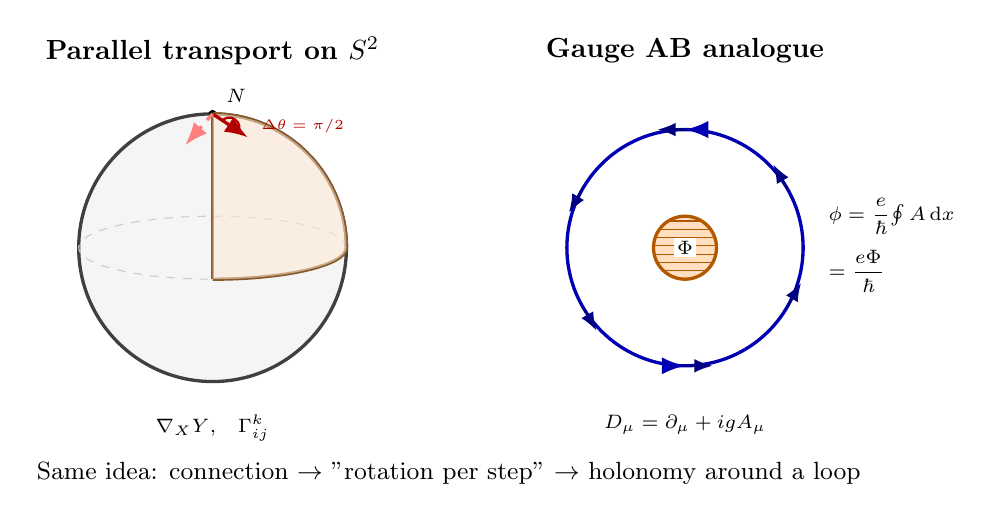
\begin{tikzpicture}[>=Latex]

  % LEFT — sphere with parallel transport triangle
  \begin{scope}[xshift=0cm]
    \node[font=\bfseries] at (0, 2.5) {Parallel transport on $S^2$};

    \draw[very thick, gray!50!black, fill=gray!8] (0, 0) circle (1.7);
    \draw[gray!40, thin, dashed] (0, 0) ellipse (1.7 and 0.4);

    % North pole
    \fill (0, 1.7) circle (0.05);
    \node[font=\scriptsize, anchor=south west] at (0.05, 1.72) {$N$};

    % triangle arcs
    \draw[very thick, brown!70!black] (0, 1.7) arc (90:0:1.7);
    \draw[very thick, brown!70!black] (1.7, 0) arc (0:-90:1.7 and 0.4);
    \draw[very thick, brown!70!black] (0, -0.4) .. controls (0, 0.4) and (0, 1.0) .. (0, 1.7);

    \fill[orange!18, opacity=0.55]
      (0, 1.7) arc (90:0:1.7) arc (0:-90:1.7 and 0.4) .. controls (0, 0.4) and (0, 1.0) .. (0, 1.7) -- cycle;

    % vectors
    \draw[->, very thick, red!70!black] (0, 1.7) -- (0.45, 1.4);
    \draw[->, very thick, red!50, dashed] (0, 1.7) -- (-0.35, 1.3);

    % angle deficit
    \draw[red!70!black, thick] (0.32, 1.45) arc (-34:140:0.13);
    \node[font=\tiny, red!70!black, anchor=west] at (0.50, 1.55) {$\Delta\theta=\pi/2$};

    \node[font=\scriptsize, anchor=north] at (0, -2.0) {$\nabla_X Y$,\quad $\Gamma^k_{ij}$};
  \end{scope}

  % RIGHT — Aharonov-Bohm
  \begin{scope}[xshift=6.0cm]
    \node[font=\bfseries] at (0, 2.5) {Gauge AB analogue};

    % loop (with arrow)
    \draw[very thick, blue!70!black, postaction={decorate, decoration={markings,
      mark=at position 0.25 with {\arrow{>}},
      mark=at position 0.75 with {\arrow{>}}}}] (0, 0) circle (1.5);

    % solenoid (central magnetic flux)
    \fill[orange!25] (0, 0) circle (0.4);
    \draw[very thick, orange!70!black] (0, 0) circle (0.4);
    \fill[pattern=horizontal lines, pattern color=orange!70!black] (0, 0) circle (0.4);
    \node[font=\scriptsize, fill=white, inner sep=1pt] at (0, 0) {$\Phi$};

    % A_mu arrows along loop (small tangential)
    \foreach \angle in {30, 90, 150, 210, 270, 330}{
      \draw[->, thick, blue!50!black]
        ({1.5*cos(\angle)},{1.5*sin(\angle)}) --
        ({1.5*cos(\angle)+0.35*cos(\angle+90)},{1.5*sin(\angle)+0.35*sin(\angle+90)});
    }

    % phase pickup
    \node[font=\scriptsize, anchor=west] at (1.7, 0.4) {$\phi=\dfrac{e}{\hbar}\!\oint A\,\mathrm dx$};
    \node[font=\scriptsize, anchor=west] at (1.7, -0.3) {$=\dfrac{e\Phi}{\hbar}$};

    \node[font=\scriptsize, anchor=north] at (0, -2.0) {$D_\mu=\partial_\mu+ig A_\mu$};
  \end{scope}

  % Bottom unifying message
  \node[font=\small, anchor=north] at (3.0, -2.6)
    {Same idea: connection $\to$ "rotation per step" $\to$ holonomy around a loop};
\end{tikzpicture}
\end{document}
